\documentclass[a4paper,oneside,14pt]{extreport}

\usepackage[T2A]{fontenc}
\usepackage[utf8]{inputenc}
\usepackage[english,russian]{babel}

\usepackage{float}
\usepackage{vmargin}
\setmarginsrb{30mm}{20mm}{20mm}{20mm}{0mm}{0mm}{0mm}{15mm}

\usepackage[unicode]{hyperref}
\hypersetup{hidelinks}

\usepackage{microtype}
\sloppy

\usepackage{indentfirst}

\usepackage{titlesec}
\titleformat{\chapter}{\LARGE\bfseries}{\thechapter}{20pt}{\LARGE\bfseries}
\titleformat{\section}{\Large\bfseries}{\thesection}{20pt}{\Large\bfseries}

\usepackage{caption}

\usepackage{amsmath}
\usepackage{amssymb}

\usepackage{graphicx}
\newcommand{\img}[3]
{
	\begin{figure}[ht]
		\center{\includegraphics[width=#1]{images/#2}}
		\caption{#3}
		\label{img:#2}
	\end{figure}
}

\usepackage{listings}
\lstset{
	basicstyle=\small,
	numbers=left,
	numberstyle=\tiny,
	stepnumber=1,
	numbersep=5pt,
	showspaces=false,
	showstringspaces=false,
	showtabs=false,
	frame=false,
	tabsize=4,
	captionpos=b,
	breaklines=true,
	breakatwhitespace=true,
	escapeinside={\#*}{*)}
}

\newcommand{\code}[1]{\texttt{#1}}

\usepackage{pgfplots}
\pgfplotsset{compat=newest}

\begin{document}
	
	\begin{titlepage}
		\centering
		
		{\footnotesize \itshape Министерство науки и высшего образования Российской Федерации\\
			Федеральное государственное бюджетное образовательное учреждение 
			высшего образования
			«Московский государственный технический университет
			имени Н.Э. Баумана
			(национальный исследовательский университет)»
			(МГТУ им. Н.Э. Баумана)\\}
		
		\vspace{60mm}
		
		\textbf{ОТЧЕТ}\\
		По лабораторной работе №1 (часть 2)\\
		По курсу: "<Операционные системы">\\
		Тема: "<Функции обработчика прерывания от системного таймера. Пересчет динамических приоритетов">\\
		
		\vspace{60mm}
		
		\hspace{70mm} Студент:
		\hfill Жабин~Д.~В.\\
		\hspace{70mm} Группа:
		\hfill ИУ7-54Б\\
		\hspace{70mm} Преподаватель:
		\hfill Рязанова~Н.~Ю.\\
		
		\vfill
		Москва, 2021
	\end{titlepage}
	
	\chapter{Функции обработчика прерывания от системного таймера}
	
	\section{UNIX}
	
	\textbf{По тику:}
	\begin{itemize}
		\item Инкремент счетчика использования процессора текущим процессом.
		\item Инкремент часов и других таймеров системы.
		\item Декремент счетчика времени, оставшегося до отправки отложенных вызовов на выполнение и отправка отложенных вызовов на выполнение при достижении нулевого значения счетчика.
		\item Декремент кванта.
	\end{itemize}
	
	\textbf{По главному тику:}
	\begin{itemize}
		\item Добавление в очередь отложенных вызовов функций планировщика.
		\item Пробуждение системных процессов \code{swapper} и \code{pagedaemon}.
		\item Декремент счетчиков времени, оставшегося до посылки сигналов тревоги:
		\begin{itemize}
			\item \code{SIGALRM} --- сигнал будильника реального времени, который посылается по истечении заданного промежутка реального времени;
			\item \code{SIGPROF} --- сигнал будильника профиля процесса, который измеряет время работы процесса;
			\item \code{SIGVTALRM} --- сигнал будильника виртуального времени, который измеряет время работы процесса в режиме задачи.
		\end{itemize}
	\end{itemize}
	
	\textbf{По кванту:}
	\begin{itemize}
		\item При превышении текущим процессом выделенного кванта, посылка сигнала \code{SIGXCPU} этому процессу.
	\end{itemize}
	
	\section{Windows}
	
	\textbf{По тику:}
	\begin{itemize}
		\item Инкремент счетчика системного времени.
		\item Декремент счетчиков отложенных задач.
		\item Декремент остатка кванта текущего потока.
		\item Активация обработчика ловушки профилирования ядра.
	\end{itemize}
	
	\textbf{По главному тику:}
	\begin{itemize}
		\item Инициализация диспетчера настройки баланса путем освобождения объекта <<событие>>, на котором он ожидает.
	\end{itemize}
	\textbf{По кванту:}
	\begin{itemize}
		\item Инициализация диспетчеризации потоков добавлением соответствующего объекта DPC в очередь.
	\end{itemize}
	\chapter{Пересчет динамических приоритетов}
	\section{UNIX}
	Классическое ядро UNIX является строго невытесняемым. Это означает, что если процесс выполняется в режиме ядра, то ядро не заставит этот процесс уступить процессорное время какому-либо более приоритетному процессу. Выполняющийся процесс может освободить процессор в случае своего блокирования в ожидании ресурса, иначе он может быть вытеснен при переходе в режим задачи. Такая реализация ядра позволяет решить множество проблем синхронизации, связанных с доступом нескольких процессов к одним и тем же структурам данных ядра.
	Однако современные ядра Linux, начиная с версии 2.5, являются полностью вытесняемыми, так как должны обеспечивать работу процессов реального времени.
	\subsection{Приоритеты процессов}
	Приоритет процесса в UNIX задается числом в диапазоне от 0 до 127, причем чем меньше значение, тем выше приоритет. Приоритеты 0--49 зарезервированы ядром операционной системы, прикладные процессы могут обладать приоритетом в диапазоне от 50 до 127.
	Структура \code{proc} содержит следующие поля, относящиеся к приоритетам:
	\begin{itemize}
		\item \code{p{\_}pri} --- текущий приоритет планирования;
		\item \code{p{\_}usrpri} --- приоритет режима задачи;
		\item \code{p{\_}cpu} --- результат последнего измерения использования процессора;
		\item \code{p{\_}nice} --- фактор "<любезности">, устанавливаемый пользователем.
	\end{itemize}
	Планировщик использует поле \code{p{\_}pri} для принятия решения о том, какой процесс отправить на выполнение. Значения \code{p{\_}pri} и \code{p{\_}usrpri} идентичны, когда процесс находится в режиме задачи. Когда процесс просыпается после блокировки в системном вызове, его приоритет временно повышается. Планировщик использует \code{p{\_}usrpri} для хранения приоритета, который будет назначен процессу при переходе из режима ядра в режим задачи, а \code{p{\_}pri} --- для хранения временного приоритета для выполнения в режиме ядра.
	Ядро связывает приоритет сна (0--49) с событием или ожидаемым ресурсом, из-за которого процесс может быть заблокирован. Когда блокированный процесс просыпается, ядро устанавливает \code{p{\_}pri}, равное приоритету сна события или ресурса, на котором он был заблокирован, следовательно, такой процесс будет назначен на выполнение раньше, чем другие процессы в режиме задачи. В таблице \ref{tbl:sleeppriority} приведены значения приоритетов сна для систем 4.3BSD UNIX и SCO UNIX (OpenServer 5.0). Такой подход позволяет системным вызовам быстрее завершать свою работу. По завершении процессом системного вызова его приоритет сбрасывается в значение текущего приоритета в режиме задачи. Если при этом приоритет окажется ниже, чем приоритет другого запущенного процесса, ядро произведет переключение контекста.
	\begin{table}[H]
		\begin{center}
			\begin{tabular}{|l|p{65pt}|p{65pt}|} 
				\hline
				{Событие} & {Приоритет 4.3BSD UNIX} & {Приоритет SCO UNIX}\\
				\hline
				{Ожидание загрузки в память страницы} & 0 & 95\\
				\hline
				{Ожидание индексного дескриптора} & 10 & 88\\
				\hline
				{Ожидание ввода--вывода} & 20 & 81 \\
				\hline
				{Ожидание буфера} & 30 & 80\\
				\hline
				{Ожидание терминального ввода} & 30 & 75\\
				\hline
				{Ожидание терминального вывода} & 30 & 74\\
				\hline
				{Ожидание завершения выполнения} & 30 & 73\\
				\hline
				{Ожидание события} & 40 & 66\\
				\hline
			\end{tabular}
		\end{center}
		\caption{Системные приоритеты сна}
		\label{tbl:sleeppriority}
	\end{table}
	Приоритет в режиме задачи зависит от "<любезности"> и последней измеренной величины использования процессора. Степень любезности --- это число в диапазоне от 0 до 39 со значением 20 по умолчанию. Степень любезности называется так потому, что одни пользователи могут быть поставлены в более выгодные условия другими пользователями посредством увеличения кем-либо из последних значения уровня любезности для своих менее важных процессов.
	Системы разделения времени стараются выделить процессорное время таким образом, чтобы все процессы системы получили его в примерно равных количествах, что требует слежения за использованием процессора. Поле \code{p{\_}cpu} содержит величину последнего измерения использования процессора процессом. При создании процесса это поле инициализируется нулем. На каждом тике обработчик таймера увеличивает \code{p{\_}cpu} на единицу для текущего процесса, вплоть до максимального значения --- 127. Каждую секунду ядро вызывает процедуру \code{schedcpu}, которая уменьшает значение \code{p{\_}cpu} каждого процесса исходя из фактора "<полураспада">. В 4.3 BSD для расчета применяется формула
	\[
	decay = \frac{2*load{\_}average}{2*load{\_}average + 1},
	\]
	где load{\_}average --- это среднее количество процессов в состоянии готовности за последнюю секунду.
	Кроме того, процедура \code{schedcpu} также пересчитывает приоритеты режима задачи всех процессов по формуле
	\[
	{p_usrpri} = PUSER + \frac{p{\_}cpu}{4} + 2*{p{\_}nice},
	\]
	где PUSER --- базовый приоритет в режиме задачи, равный 50.
	Таким образом, если процесс до вытеснения другим процессом использовал большое количество процессорного времени, его \code{p{\_}cpu} будет увеличен, что приведен к увеличению значения \code{p{\_}usrpri}, и, следовательно, к понижению приоритета.
	Чем дольше процесс простаивает в очереди на выполнение, тем меньше его \code{p{\_}cpu}. Это позволяет предотвратить зависания низкоприоритетных процессов. Если процесс б\'{о}льшую часть времени выполнения тратит на ожидание ввода-вывода, то он остается с высоким приоритетом.
	В системах разделения времени фактор использования процессора обеспечивает справедливость при планировании процессов. Фактор полураспада обеспечивает экспоненциально взвешенное среднее значение использования процессора в течение функционирования процесса. Формула, применяемая в SVR3 имеет недостаток: вычисляя простое экспоненциальное среднее, она способствует росту приоритетов при увеличении загрузки системы.
	\section{Windows}
	В системе Windows реализовано вытесняющее планирование на основе уровней приоритета, при котором выполняется готовый поток с наивысшим приоритетом.
	Процессорное время, выделенное на выполнение потока, называется квантом. Если поток с более высоким приоритетом готов к выполнению, то он вытесняет текущий поток, даже если квант текущего потока не истек.
	В Windows за планирование отвечает совокупность процедур ядра, называемая диспетчером ядра. Диспетчеризация может быть вызвана, если:
	\begin{itemize}
		\item поток готов к выполнению;
		\item истек квант текущего потока;
		\item поток завершается или переходит в состояние ожидания;
		\item изменился приоритет потока;
		\item изменилась привязка потока к процессору.
	\end{itemize}
	\subsection{Приоритеты потоков}
	В системе предусмотрено 32 уровня приоритетов: уровни реального времени (16--31), динамические уровни (1--15) и системный уровень (0). 
	Уровни приоритета потоков назначаются Windows API и ядром операционной системы.
	Windows API сортирует процессы по классам приоритета, которые были назначены при их создании:
	\begin{itemize}
		\item реального времени --- Real-time (4);
		\item высокий --- High (3);
		\item выше обычного --- Above Normal (6);
		\item обычный --- Normal (2);
		\item ниже обычного --- Below Normal (5);
		\item простой --- Idle (1).
	\end{itemize}
	Затем назначается относительный приоритет потоков в рамках процессов:
	\begin{itemize}
		\item критичный по времени --- Time-critical (15);
		\item наивысший --- Highest (2);
		\item выше обычного --- Above-normal (1);
		\item обычный --- Normal (0);
		\item ниже обычного --- Below-normal (-1);
		\item низший --- Lowest (-2);
		\item простой --- Idle (-15).
	\end{itemize}
	Относительный приоритет --- это приращение к базовому приоритету процесса.
	Соответствие между приоритетами Windows API и ядра системы приведено в таблице \ref{tbl:priority}.
	\begin{table}[H]
		\begin{center}
			\begin{tabular}{|l|p{45pt}|p{45pt}|p{45pt}|p{45pt}|p{45pt}|p{45pt}|} 
				\hline
				{} & Real-time & High & Above-Normal & Normal & Below-Normal & Idle\\
				\hline
				Time Critical & 31 & 15 & 15 & 15 & 15 & 15 \\
				\hline
				Highest & 26 & 15 & 12 & 10 & 8 & 6 \\
				\hline
				Above Normal & 25 & 14 & 11 & 9 & 7 & 5 \\
				\hline
				Normal & 24 & 13 & 10 & 8 & 6 & 4 \\
				\hline
				Below Normal & 23 & 12 & 9 & 7 & 5 & 3 \\
				\hline
				Lowest & 22 & 11 & 8 & 6 & 4 & 2 \\
				\hline
				Idle & 16 & 1 & 1 & 1 & 1 & 1 \\
				\hline
			\end{tabular}
		\end{center}
		\caption{Соответствие между приоритетами Windows API и ядра Windows}
		\label{tbl:priority}
	\end{table}
	Каким бы образом ни формировался приоритет потока, с точки зрения планировщика Windows важно только значение приоритета.
	Процесс обладает только базовым приоритетом, тогда как поток имеет базовый, который наследуется от приоритета процесса, и текущий приоритет. Операционная система может на короткие интервалы времени повышать приоритеты потоков из динамического диапазона, но никогда не регулирует приоритеты потоков в диапазоне реального времени.
	Приложения пользователя запускаются, как правило, с базовым приоритетом Normal. Некоторые системные процессы имеют приоритет выше 8, следовательно, это гарантирует, что потоки в этих процессах будут запускаться с более высоким приоритетом.
	Система повышает приоритет текущего потока в следующих случаях:
	\begin{itemize}
		\item по завершении операции ввода-вывода;
		\item по окончании ожидания на событии или семафоре исполнительной системы;
		\item по окончании ожидания потоками активного процесса;
		\item при пробуждении GUI-потоков из-за операции с окнами;
		\item если поток, готовый к выполнению, задерживается из-за нехватки процессорного времени.
	\end{itemize}
	Повышение приоритета применяется только к потокам из динамического диапазона (1--15) и, независимо от приращения, приоритет потока не может оказаться выше 15.
	\subsection{Повышение приоритета по завершении операции ввода-вывода}
	По окончании определенных операций ввода-вывода Windows временно повышает приоритет потоков и потоки, ожидающие завершения этих операций, имеют больше шансов немедленно возобновить выполнение и обработать полученные от устройств ввода-вывода данные.
	Драйвер устройства ввода-вывода через функцию \code{IoCompleteRequest} указывает на необходимость повышения приоритета после выполнения соответствующего запроса.
	В таблице \ref{tbl:priorityinc} приведены приращения приоритетов.
	\begin{table}[H]
		\begin{center}
			\begin{tabular}{|p{100mm}|l|} 
				\hline
				Устройство & Приращение \\	
				\hline
				Диск, CD-ROM, параллельный порт, видео & 1 \\
				\hline
				Сеть, почтовый ящик, именованный канал, последовательный порт & 2 \\
				\hline
				Клавиатура, мышь & 6 \\
				\hline
				Звуковая плата & 8 \\
				\hline
			\end{tabular}
		\end{center}
		\caption{Рекомендованные приращения приоритета}
		\label{tbl:priorityinc}
	\end{table}
	Приоритет потока всегда повышается относительно базового приоритета. На рисунке \ref{fig:dp} показано, что после повышения приоритета поток в течение одного кванта выполняется с повышенным приоритетом, а затем приоритет снижается на один уровень с каждым последующим квантом. Цикл продолжается до тех пор, пока приоритет не снизится до базового.
	\begin{figure}[H]
		\centering
		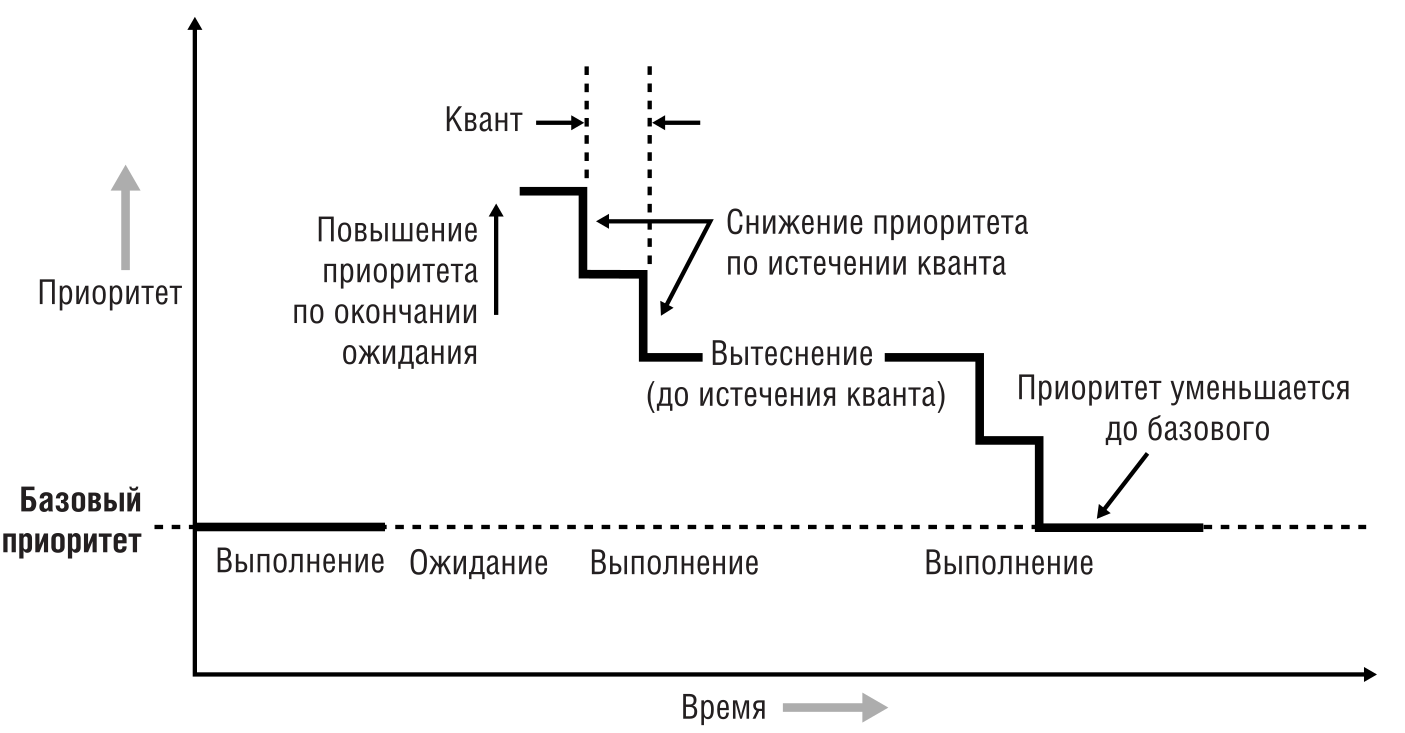
\includegraphics[scale=0.3]{images/priority}
		\caption{Динамическое изменение приоритета}
		\label{fig:dp}
	\end{figure}
	\subsection{Повышение приоритета по окончании ожидания на событии или семафоре}
	Если ожидание потока на событии системы или семафоре успешно завершается из-за вызова \code{SetEvent}, \code{PulseEvent} или \code{ReleaseSemaphore}, его приоритет повышается на 1.
	Такая регулировка, как и в случае с окончанием операции ввода-вывода, позволяет более равномерно распределить процессорное время --- потокам, блокируемым на событиях, процессорное время требуется реже, чем остальным. В данном случае действуют те же правила повышения приоритета.
	К потокам, пробуждающимся в результате установки события вызовом функций \code{NtSetEventBoostPriority} и \code{KeSetEventBoostPriority}, повышение приоритета применяется особым образом.
	\subsection{Повышение приоритета по окончании ожидания потоками активного процесса}
	Если поток в активном процессе завершает ожидание на объекте ядра, функция ядра \code{KiUnwaitThread} повышает его текущий приоритет на величину значения \code{PsPrioritySeparation}. \code{PsPriorituSeparation} --- это индекс в таблице квантов, с помощью которой выбираются величины квантов для потоков активных процессов. Какой процесс является в данный момент активным, определяет подсистема управления окнами.
	В данном случае приоритет повышается для создания преимуществ интерактивным приложениям по окончании ожидания, в результате чего повышаются шансы на немедленное возобновление потока приложения.
	Важной особенностью данного вида повышения приоритета является то, что он поддерживается всеми системами Windows и не может быть отключен даже функцией \code{SetThreadPriorityBoost}.
	\subsection{Повышение приоритета при пробуждении GUI-потоков}
	Приоритет потоков окон пользовательского интерфейса повышается на 2 после их пробуждения из-за активности подсистемы управления окнами. Приоритет повышается по той же причине, что и в предыдущем случае --- для увеличения отзывчивости интерактивных приложений.
	\subsection{Повышение приоритета при нехватке процессорного времени}
	Раз в секунду диспетчер настройки баланса --- системный поток, предназначенный для выполнения функций управления памятью --- сканирует очереди готовых потоков и ищет потоки, которые находятся в состоянии готовности в течение примерно 4 секунд. Диспетчер настройки баланса повышает приоритет таких потоков до 15. Причем в Windows 2000 и Windows XP квант потока удваивается относительно кванта процесса, а в Windows Server 2003 квант устанавливается равным 4 единицам. По истечении кванта приоритет потока снижается до исходного уровня. Если потоку все еще не хватило процессорного времени, то после снижения приоритета он возвращается в очередь готовых процессов. Через 4 секунды он может снова получить повышение приоритета.
	Чтобы свести к минимуму расход процессорного времени, диспетчер настройки баланса сканирует только 16 готовых потоков за раз, а повышает приоритет не более чем у 10 потоков за раз.
	Диспетчер настройки баланса не решает всех проблем с приоритетами потоков, однако позволяет потокам, которым не хватает процессорного времени, получить его.
	\subsection{Уровни запросов прерываний}
	Windows использует схему приоритетов прерываний, называемую уровни запросов прерываний (IRQL). Внутри ядра IRQL представляются в виде номеров до 0 до 31 для систем x86. Ядро определяет стандартный набор IRQL для программных прерываний, а HAL связывает IRQL с номерами аппаратных прерываний (см. рис. \ref{fig:ts}).
	\begin{figure}[H]
		\centering
		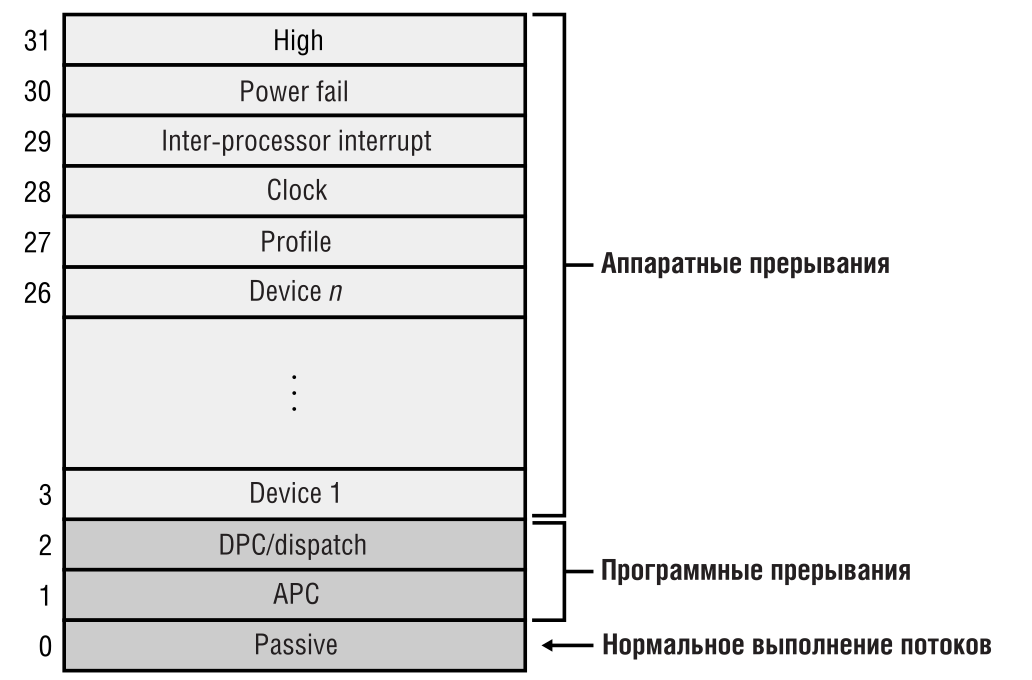
\includegraphics[scale=0.45]{images/irql}
		\caption{Уровни запросов прерываний}
		\label{fig:ts}
	\end{figure}
	Прерывания обслуживаются в порядке их приоритета. Прерывания с б\'{о}льшим приоритетом вытесняют прерывания с меньшим приоритетом.
	При возникновении прерывания с высоким приоритетом процессор сохраняет информацию о состоянии прерванного потока и активизирует сопоставленный с данным прерыванием диспетчер ловушки. Последний повышает IRQL и вызывает процедуру обслуживания прерывания --- ISR. После выполнения ISR диспетчер прерывания понижает IRQL до исходного уровня и загружает сохраненные ранее данные о состоянии машины. Прерванный поток возобновляется с той точки, где он был прерван. Когда ядро понижает IRQL, могут начать обрабатываться ранее замаскированные прерывания с более низким приоритетом. Тогда вышеописанный процесс повторяется ядром для обработки и этих прерываний.
	\chapter*{Заключение}
	\addcontentsline{toc}{chapter}{Заключение}
	Операционные системы UNIX и Windows являются системами разделения времени с вытеснением. В связи с этим обработчики прерываний от системного таймера в них выполняют схожие функции:
	\begin{itemize}
		\item инкремент счетчика системного времени;
		\item декремент кванта;
		\item добавление функций планировщика в очередь отложенных вызовов;
		\item декремент счетчиков времени, оставшегося до выполнения отложенных вызовов;
		\item отправка отложенных вызовов на выполнение.
	\end{itemize}
	Декремент кванта является основной функцией обработчика прерывания от системного таймера.
	Классическое ядро UNIX является строго невытесняющим. Ядра Linux, начиная с версии 2.5, и ядра операционных систем Windows являются полностью вытесняющими для обеспечения работы процессов реального времени.
\end{document}